% LTeX: language=fr
%%%%%%%%%%%%%%%%%%%%%%%%%%%%%%%%%%%%%%%%%%%%%%%%%%%%%%%%%%%%%%%%%%%%%%%%%%%%
%%%%%                          ANNEXE 7                               %%%%%%
%%%%%%%%%%%%%%%%%%%%%%%%%%%%%%%%%%%%%%%%%%%%%%%%%%%%%%%%%%%%%%%%%%%%%%%%%%%%

%\appendix
%\renewcommand\chaptername{Annexe~}
\phantomsection 

\lhead[\fancyplain{}{\leftmark}]%Pour les pages paires \bfseries
      {\fancyplain{}{}} %Pour les pages impaires
\chead[\fancyplain{}{}]%
      {\fancyplain{}{}}
\rhead[\fancyplain{}{}]%Pour les pages paires 
      {\fancyplain{}{\rightmark}}%Pour les pages impaires \bfseries
\lfoot[\fancyplain{}{}]%
      {\fancyplain{}{}}
\cfoot[\fancyplain{}{\thepage}]%\bfseries
      {\fancyplain{}{\thepage}} %\bfseries
\rfoot[\fancyplain{}{}]%
     {\fancyplain{}{\scriptsize}}


%%%%%%%%%%%%%%%%%%%%%%%%%%%%%%%%%%%%%%%%%%%%%%%%%%%%%%%%%%%%%%%%%%%%%%%%%%
%%%%%                      Start part here                          %%%%%%
%%%%%%%%%%%%%%%%%%%%%%%%%%%%%%%%%%%%%%%%%%%%%%%%%%%%%%%%%%%%%%%%%%%%%%%%%%

\chapter{Cinématique de pliage des VH avec les gaines rigides}
\label{Ann:Annexe7_cinematique_M-VH}

\minitoc
\newpage

Lorsque le rayon de la GR est supérieur au bras de levier de pliage $a$ nécessaire pour satisfaire $\Delta\theta$, il se produit un changement dans la configuration de pliage de la VH avec l'évolution du point de contact entre la VH et M (\ref{fig:cinematique_VH_mini}). Les sections qui suivent détaillent les calculs ayant servi pour la modélisation de la cinématique de pliage avec l'influence de la GR.
%/!\/!\/!\/!\/!\/!\/!\/!\/!\/!\/!\/!\/!\/!\/!\/!\/!\/!\/!\/!\/!\/!\/!\/!\ 
\section{Contact latéral}
\label{subsubsec:4.3.2.a_Avant saut}
%/!\/!\/!\/!\/!\/!\/!\/!\/!\/!\/!\/!\/!\/!\/!\/!\/!\/!\/!\/!\/!\/!\/!\/!\
%%%%%%%%%%%%%%%%
\begin{table}[!htbp]
   \centering
   \captionsetup{justification=centering}
   \rowcolors[]{2}{black!8}{}{
      \begin{tabular}{m{0.6\textwidth} c c }
         \rowcolor{blue!10}
         \toprule
         \textbf{Nom de la variable}                             & \textbf{Symbole} & \textbf{Entrée(E)/Sortie(S)} \\
         \midrule
         Diamètre extérieur de la gaine rigide                          & $D_{gr}$            & E                            \\
         Angle de VH avant le contact M-VH                       & $\theta_0$       & E                            \\
         \textbf{Angle de VH avant durant le contact M-VH}       & $\theta_f$       & E / S                        \\
         Position de M                                           & $x_{m}$          & E                            \\
         Raideur de la VH                                        & $K_{VH}$         & E                            \\
         \textbf{Position de M à l'équilibre pour l'OBVH$_{ag}$} & $x_{0,vh}$       & E / S                        \\
         \textbf{Position de M à l'équilibre pour l'OB$_{ag}$}   & $x_0$            & E / S                        \\
         Abscisse de C pour $\theta=\theta_0$                    & $x_{\theta 0}$   & S                            \\
         Abscisse de C pour $\theta=\theta_f$                    & $x_{\theta f}$   & S                            \\
         Bras de levier de pliage de VH au contact latéral       & $a$              & S                            \\
         Abscisse limite de M avant l'apparition du contact supérieur   & $x_{ms}$         & S                            \\
         \bottomrule
      \end{tabular}}
   \caption{Définition des paramètres géométriques d'entrée et de sortie dans la configuration du contact latéral M-VH}
   \label{tab:parametres_avant_saut}
\end{table}
%%%%%%%%%%%%%%%%%%%%%      
Durant le contact latéral, le point $C$ se trouve obligatoirement sur une arête de M, suivant l'orientation de la VH et de M. Sur la configuration présentée sur les figures de cette annexe, ainsi que sur les essais expérimentaux de lâcher avec VH, $C$ se trouve sur l'arrête supérieure droite de M. Les variables définissant la géométrie autour du contact M-VH sont listées dans le tableau \ref{tab:parametres_avant_saut}.

Il s'agit à présent de définir les variables d'entrée et de sortie du système d'équations issu de la configuration de contact latéral. Ceux-ci représentent respectivement les paramètres connus et ceux qu'on cherche à évaluer au travers du système d'équations.

Les paramètres que nous connaissons peuvent être de deux natures. Ils sont soit fixés par la géométrie propre des composants, soit imposés par le cahier des charges. La géométrie de la GR fixe le diamètre $D_{gr}$. Le CdC hydraulique de la valve impose $\theta_0$, ainsi que la plage d'évolution $\Delta\theta$ souhaitée lorsque $x_m\in [0;\pm x_{0,vh}]$ pour assurer $(r_{Cf})_{min}=10$. Le bras de levier de pliage $a$ calculé par l'équation \ref{eq:theta=f(x_m)} est valide seulement si le rapport entre les rayons de GR et de VH est proche de 1. Expérimentalement, ce rapport est ici de 4 et donc $a$ est à recalculer avec cette nouvelle configuration. En prenant donc en compte les aspects statiques (eq. \ref{eq:x_0f} - \ref{eq:equilibre_statique}) et les aspects cinématiques (eq. \ref{eq:f} - \ref{eq:xt}), on peut calculer la valeur des paramètres de sortie désirés à partir des variables d'entrée qui sont définis dans le tableau \ref{tab:parametres_avant_saut}.
%%%%%%%%%%%%%%%%%%%%%%%%%%%%%%%%%%%%	
\begin{subnumcases}{S_{av}~~}
$$
f = \dfrac{D_{gr}}{2}\ (1-\cos(\theta))
$$
\label{eq:f}\\
$$
m = \dfrac{D_{gr}}{2}\ sin(\theta)
$$
\label{eq:m}\\
$$
k = a - m
$$
\label{eq:k}\\
$$
\varphi = \arctan\biggl(\dfrac{f}{k}\biggr)
$$
\label{eq:varphi_cin}\\
$$
j = \dfrac{k}{\cos(\varphi)}
$$
\label{eq:j}\\
$$
h = \dfrac{k}{\cos(\theta)}
$$
\label{eq:h}\\
$$
c = h \sin(\theta)
$$
\label{eq:c}\\
$$
x_m = c + f
$$
\label{eq:xt}
\end{subnumcases} 
\begin{subnumcases}{}
$$
   x_{0,vh} = x_{\theta 0} - x_{\theta f}
$$ \label{eq:x_0f}\\
\vspace{2cm}
$$
\dfrac{2K\ {{x_{0}}}^2}{L^2}\biggl(\dfrac{{x_{0,vh}}^2}{{x_{0}}^2}-1\biggr)x_{0,vh}
\ +\ \dfrac{K_{VH}}{a}\theta
\ =\ 0 
$$ \label{eq:equilibre_statique}
\end{subnumcases}
%%%%%%%%%%%%%%%%%%%%%%%%%%%%%%%%%%%%
%%%%%%%%%%%%%%%%%%%%%%%%%%%%%%%%%%%%	
\begin{figure}[!htb]
\begin{center}
 \captionsetup{justification=centering} 
   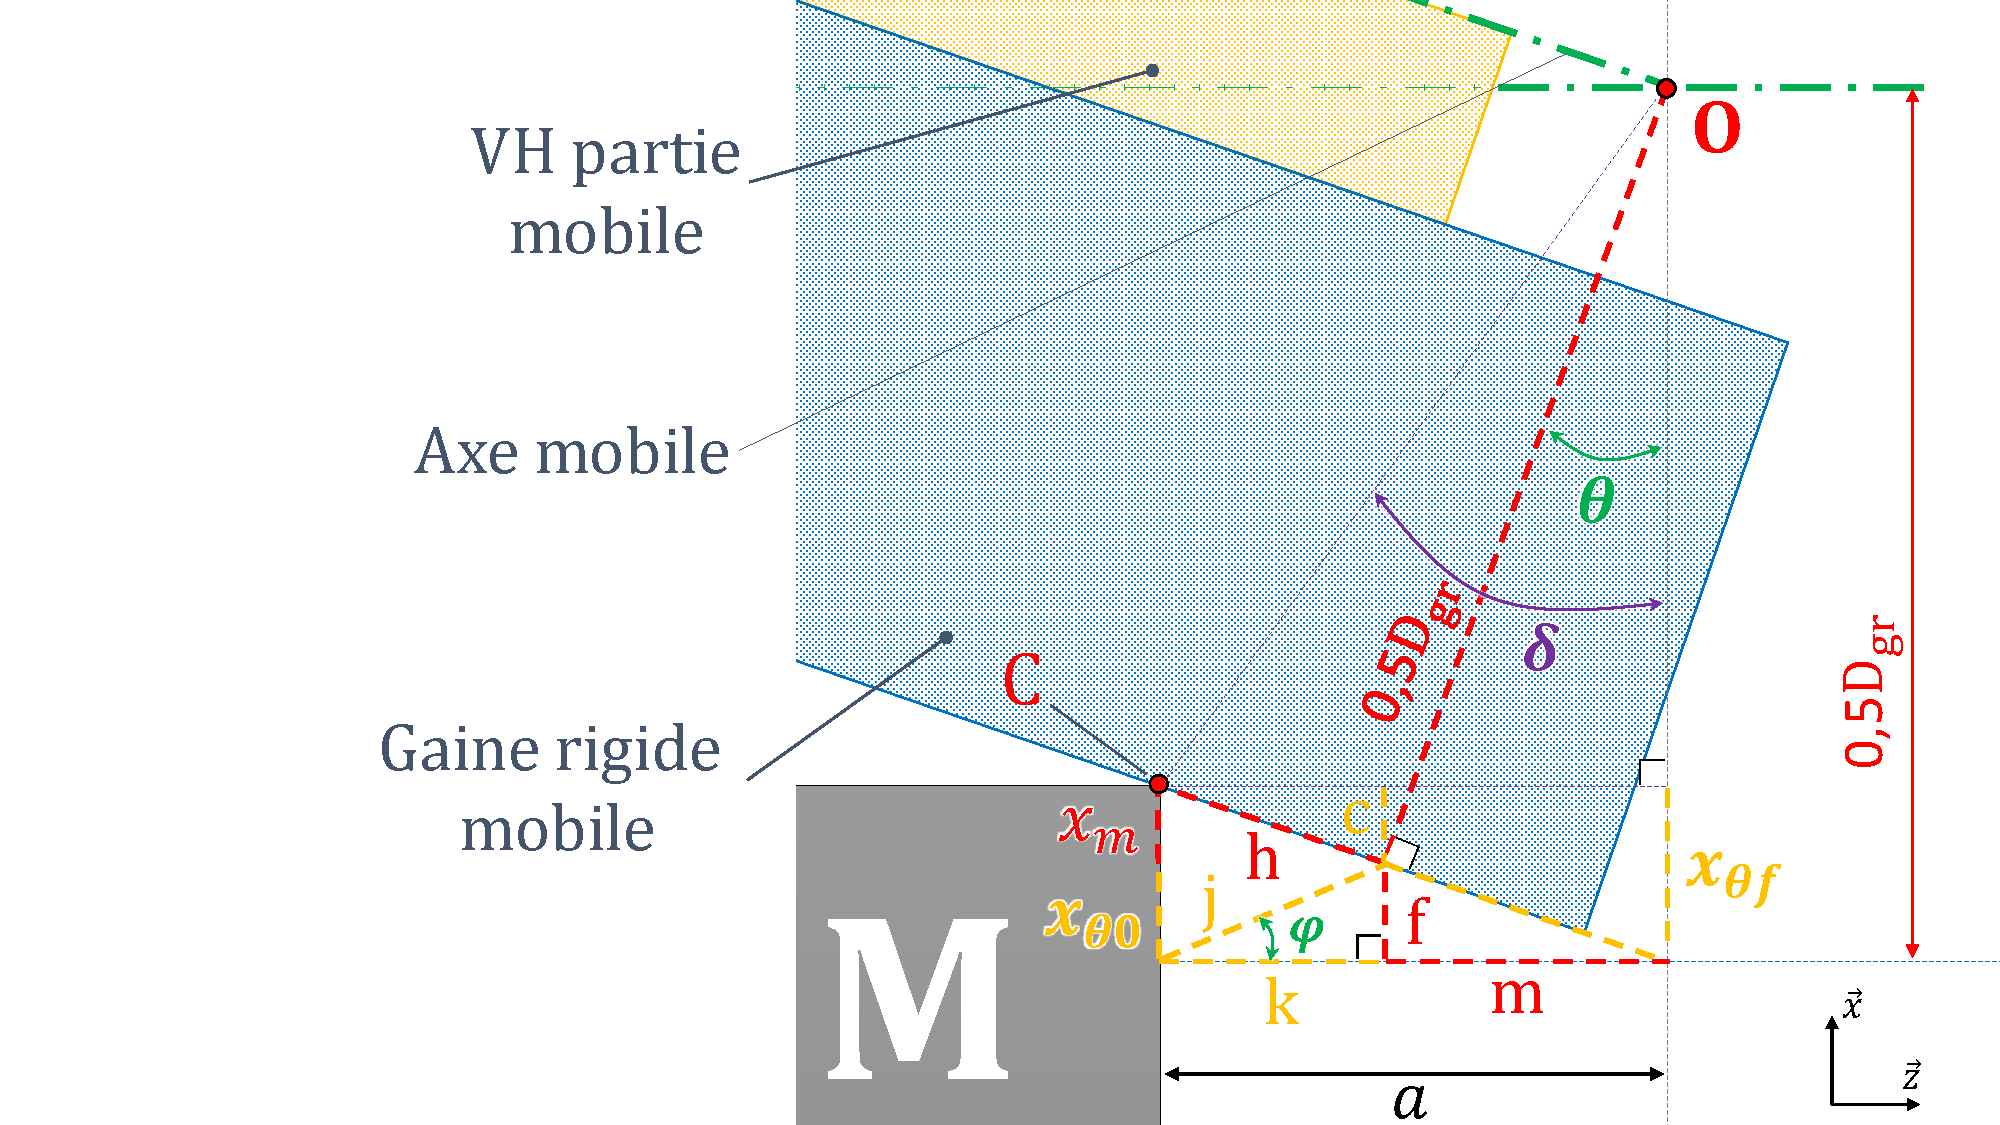
\includegraphics[trim={6cm 0cm 0cm 0cm},clip,width=0.8\textwidth]{../Chap6/Figure/cinematique_pliage_VH_lacher_calculs.pdf}
   \caption{Cinématique du contact M-VH latéral}
   \label{fig:cinematique_pliage_VH_lacher}
\end{center}	
\end{figure}    
%%%%%%%%%%%%%%%%%%%%%%%%%%%%%%%%%%%%	

La figure \ref{fig:cinematique_pliage_VH_lacher} montre le schéma de définition des paramètres dans la configuration de contact \emph{latéral}. On dénombre trois paramètres d'entrée/sortie caractéristiques du fonctionnement du système, repérés en gras dans le tableau \ref{tab:parametres_avant_saut}. L'un devra obligatoirement être fixé pour permettre l'estimation des deux autres. Dépendamment du CdC du système, ainsi que des moyens technologiques qu'on possède, on choisira un scénario de dimensionnement plutôt qu'un autre. Les conséquences d'imposer ou non l'un ou l'autre des paramètres caractéristiques sont les suivantes :
\begin{itemize}[label=$\bullet$]
   \item Imposer $\theta_f$, et $\Delta\theta$ par extension, permettra de prédire le comportement hydraulique de la valve hydraulique avec GR (VH$_{ag}$). De plus, cela fixera la raideur $K_{vh}(\theta_f)$ d'après les essais statiques réalisés sur le tube plastifié considéré.
   \item Imposer $x_{0}$, la hauteur de flambement de l'OB avant que la VH$_{ag}$ ne vienne en contact avec celui-ci, permettra de s'assurer qu'il soit plus petit que $x_{0,max}$ (tab. \ref{tab:x0max}). Cela maximisera l'efficacité de conversion en évitant une réduction du coefficient de couplage électromécanique suite à l'apparition de flambements locaux sur les portions fines des LF de l'OB lors des phases de compression.
   \item Imposer la hauteur de flambement $x_{0,vh}$ de l'OBVH$_{ag}$ lorsque la VH$_{ag}$ est implémentée sur l'OB, permettrait de s'assurer du niveau énergétique nécessaire pour faire basculer M d'une position d'équilibre à l'autre.
\end{itemize}
Il sera judicieux pour notre application d'avoir le contrôle sur le niveau d'énergie nécessaire pour le basculement de M au passage de 0, afin de l'adapter à l'énergie disponible dans l'oreille. Par ailleurs, le bon fonctionnement du système nécessite une commutation hydraulique efficace et donc imposer $\Delta\theta$ est un impératif pour notre application. L'OB pourra en dernier lieu être dimensionné afin d'admettre une limite $x_{0m}$ suffisante pour supporter les contraintes induites par le niveau énergétique d'entrée.

Les deux positions $x_{\theta f}$ et $x_{\theta 0}$ de M sont respectivement calculé à partir de l'évaluation du système d'équation cinématique $S_{lat}$ pour la borne supérieure et pour la borne inférieure de l'intervalle d'angle $\Delta\theta$.

Le système d'équations $S_{lat}$ est cependant valable à la condition que la distance $h$ soit positive. En effet, lorsque $\theta$ s'approche de $\delta$, la distance $h$ tend vers 0. En traçant alors l'évolution de $h$ et $\theta$ suivant $x_m$ pour un bras de levier $a$ inférieur à $Dg/2$ (fig. \ref{fig:theta_saut}), on s'aperçoit que lorsque h tend vers 0 (fig. \ref{fig:cinematique_pliage_VH_lacher}), la variation de $\theta$ en fonction de $x_m$ devient de plus en plus importante.
%%%%%%%%%%%%%%%%%%%%%%%%%%%%%%%%%%%%	
\begin{figure}[!htb]
\begin{center}
 \captionsetup{justification=centering} 
   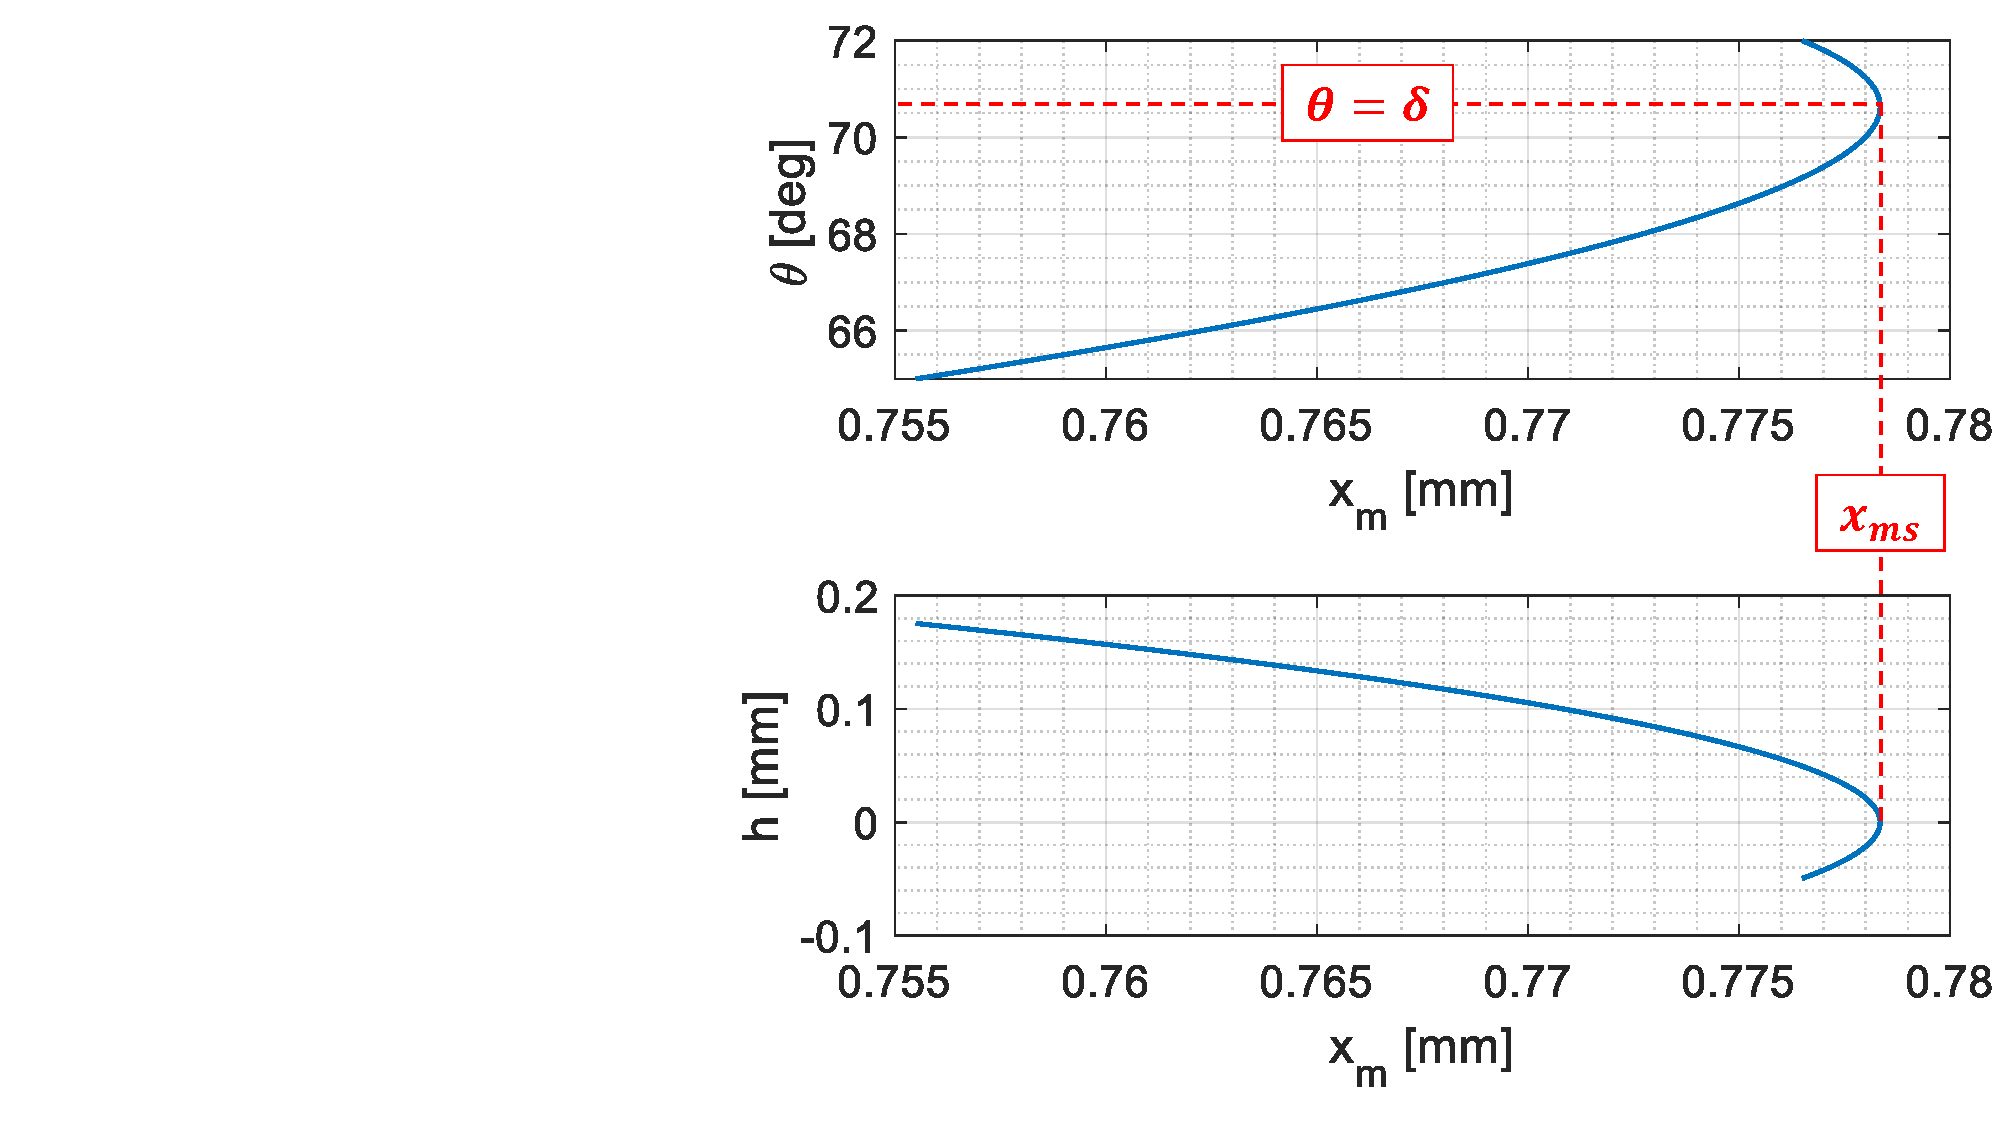
\includegraphics[trim={12cm 0cm 0cm 0cm},clip,width=0.55\textwidth]{../Chap6/Figure/theta_saut.pdf}
   \caption{Évolution de $h$ et $\theta$ en fonction de $x_m$ lorsque $h$ tend vers 0}
   \label{fig:theta_saut}
\end{center}	
\end{figure}    
%%%%%%%%%%%%%%%%%%%%%%%%%%%%%%%%%%%%

Les valeurs de $\theta$ au-delà de $\delta$ n'ont pas de sens physique. En réalité, c'est à ce moment-là que se produit le changement de configuration de contact qui passe du latéral (fig. \ref{fig:cinematique_VH_avant-saut_mini}) au supérieur (fig. \ref{fig:cinematique_VH_après-saut_mini}). On définit alors $x_{ms}$ la position maximale de M fixant la limite du domaine de validité du système d'équations $S_{lat}$. On peut évaluer $x_{ms}$ avec le système d'équations $S_{lat}$ car on connaît la valeur de $\theta(x_{ms})$ qui s'exprime par l'équation \ref{eq:theta_max_av_saut}
\begin{equation}
\theta(x_{ms})\ =\ \delta(x_{ms})\ =\ \arctan\biggl(\dfrac{2a}{D_{gr}}\biggr)
\label{eq:theta_max_av_saut}
\end{equation} 
%/!\/!\/!\/!\/!\/!\/!\/!\/!\/!\/!\/!\/!\/!\/!\/!\/!\/!\/!\/!\/!\/!\/!\/!\
\section{Contact supérieur}
\label{subsubsec:4.3.2.b_Apres saut}
%/!\/!\/!\/!\/!\/!\/!\/!\/!\/!\/!\/!\/!\/!\/!\/!\/!\/!\/!\/!\/!\/!\/!\/!\
%%%%%%%%%%%%%%%%%
\begin{table}[!htbp]
   \centering
   \rowcolors[]{2}{black!8}{}{
         \begin{tabular}{m{0.6\textwidth} c c }
         \rowcolor{blue!10}    
\textbf{Nom de la variable}                  & \textbf{Symbole}   & \textbf{Entrée(E)/Sortie(S)}    \\
\hline \hline
Diamètre extérieur de la gaine	     	     &  $D_{gr}$ 			& E	\\ 
Abscisse de C pour $\theta=\theta_0$   		 &  $x_{\theta_0}$  & E	\\
Bras de levier de pliage de VH avant saut  	 &	$a$   			& E	\\
Différence de longueur entre GR mobile et kapton mobile  								 & $b$ 		& E \\ 
Abscisse de C pour $\theta=\theta_f$   		 &	$x_{\theta_f}$  & S	\\ 
Angle de VH durant le contact M-VH après saut&	$\theta_s$ 	    & S	\\ 
Bras de levier de pliage de VH après saut  	 &	$a_s$   		& S	\\ \hline
         \end{tabular}}
     \caption{Définition des paramètres géométriques d'entrée et de sortie du système d'équation $S_{sup}$(\ref{eq:S_ap}) après saut}
     \label{tab:parametres_apres_saut}
\end{table} 
%%%%%%%%%%%%%%%%%%%%%          
Lorsque $a$ est plus petit que $D_{gr}/2$, comme c'est le cas dans le réglage du banc expérimental présenté à la figure \ref{fig:deplacement_zlat}, on constate que la variation de $\theta$ suivant $x_m$ devient de plus en plus importante lorsque $\theta$ approche de la valeur de $\delta$. En effet, le contact supérieur apparaît et change ainsi la configuration de pliage de la VH suivant les schémas présentés sur la figure \ref{fig:cinematique_pliage_VH_lacher_calculs_saut}. 
\begin{equation}
\delta_s = \theta_s = \arctan\biggl(\dfrac{2a}{D_{gr}}\biggr)
\label{eq:delta_s} 
\end{equation}
On va retrouver trois cas de figure, illustrés sur la figure  \ref{fig:cinematique_pliage_VH_lacher_calculs_saut}, lorsque la configuration de contact supérieur apparaît. En effet, dépendamment de la différence de longueur $b$ (éq. \ref{eq:b_definition_annexe}) entre la partie mobile en kapton et de la GR mobile, la configuration de pliage sera différente pour un bras de levier initial $a$ identique. 
\begin{equation}
	b = \dfrac{L_t}{2} - L_{gr}
	\label{eq:b_definition_annexe}
\end{equation}

La distance entre le centre de rotation $O$ et le point de contact $C_s$ va varier en fonction de la différence de longueur $b$ et sera minimal pour $b=0$, où elle vaudra $D_{gr}$ (fig. \ref{fig:cinematique_pliage_VH_lacher_calculs_saut}). Le bras de levier $a_s$ durant le contact supérieur sera par conséquent le plus petit quand $b$ sera nul. De plus, $\theta_s$ sera différent selon $b$.
\begin{itemize}[label=$\circ$]
   \item Si $b>0$, alors $\theta_{s} < \delta_s $ (figure \ref{fig:cinematique_pliage_VH_lacher_calculs_saut_petit})
   \item Si $b=0$, alors $\theta_{s} = \delta_s $ (figure \ref{fig:cinematique_pliage_VH_lacher_calculs_saut_égal}) 
   \item Si $b<0$, alors $\theta_{s} > \delta_s $ (figure \ref{fig:cinematique_pliage_VH_lacher_calculs_saut_grand}) 
\end{itemize} 
L'inégalité $\theta_{s1} < \theta_{s2} = \delta_s < \theta_{s3}$ sera toujours vraie, quel que soit $b$.

%%%%%%%%%%%%%%%%
\begin{figure}[!htb]
   \begin{minipage}{.5\linewidth}
      \centering
      \subfloat[]{\label{fig:cinematique_pliage_VH_lacher_calculs_saut_petit}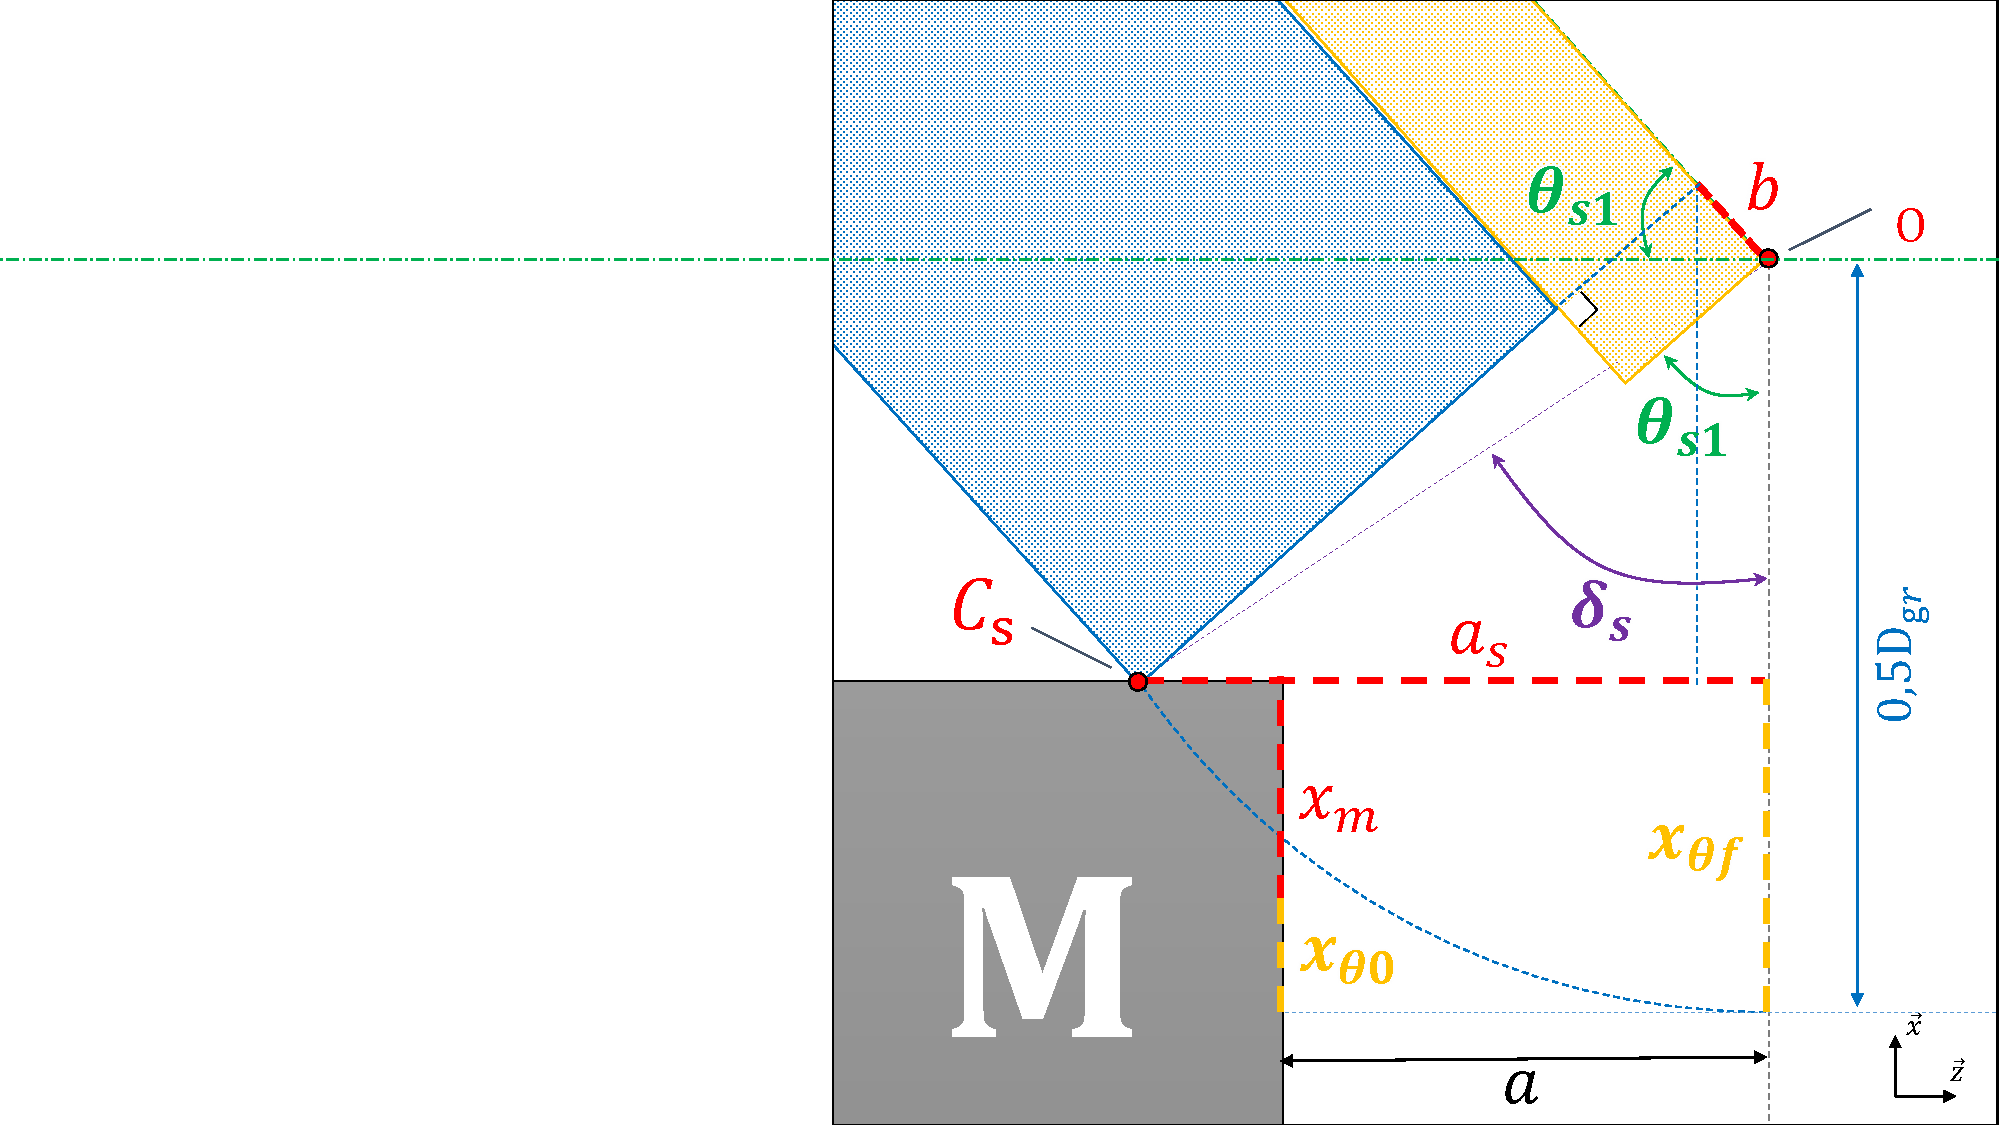
\includegraphics[trim={14cm 0cm 0cm 0cm},clip, 					                 width=.99\textwidth]{../Chap6/Figure/cinematique_pliage_VH_lacher_calculs_saut_petit.pdf}}
   \end{minipage}%
   \begin{minipage}{.5\linewidth}
      \centering
      \subfloat[]{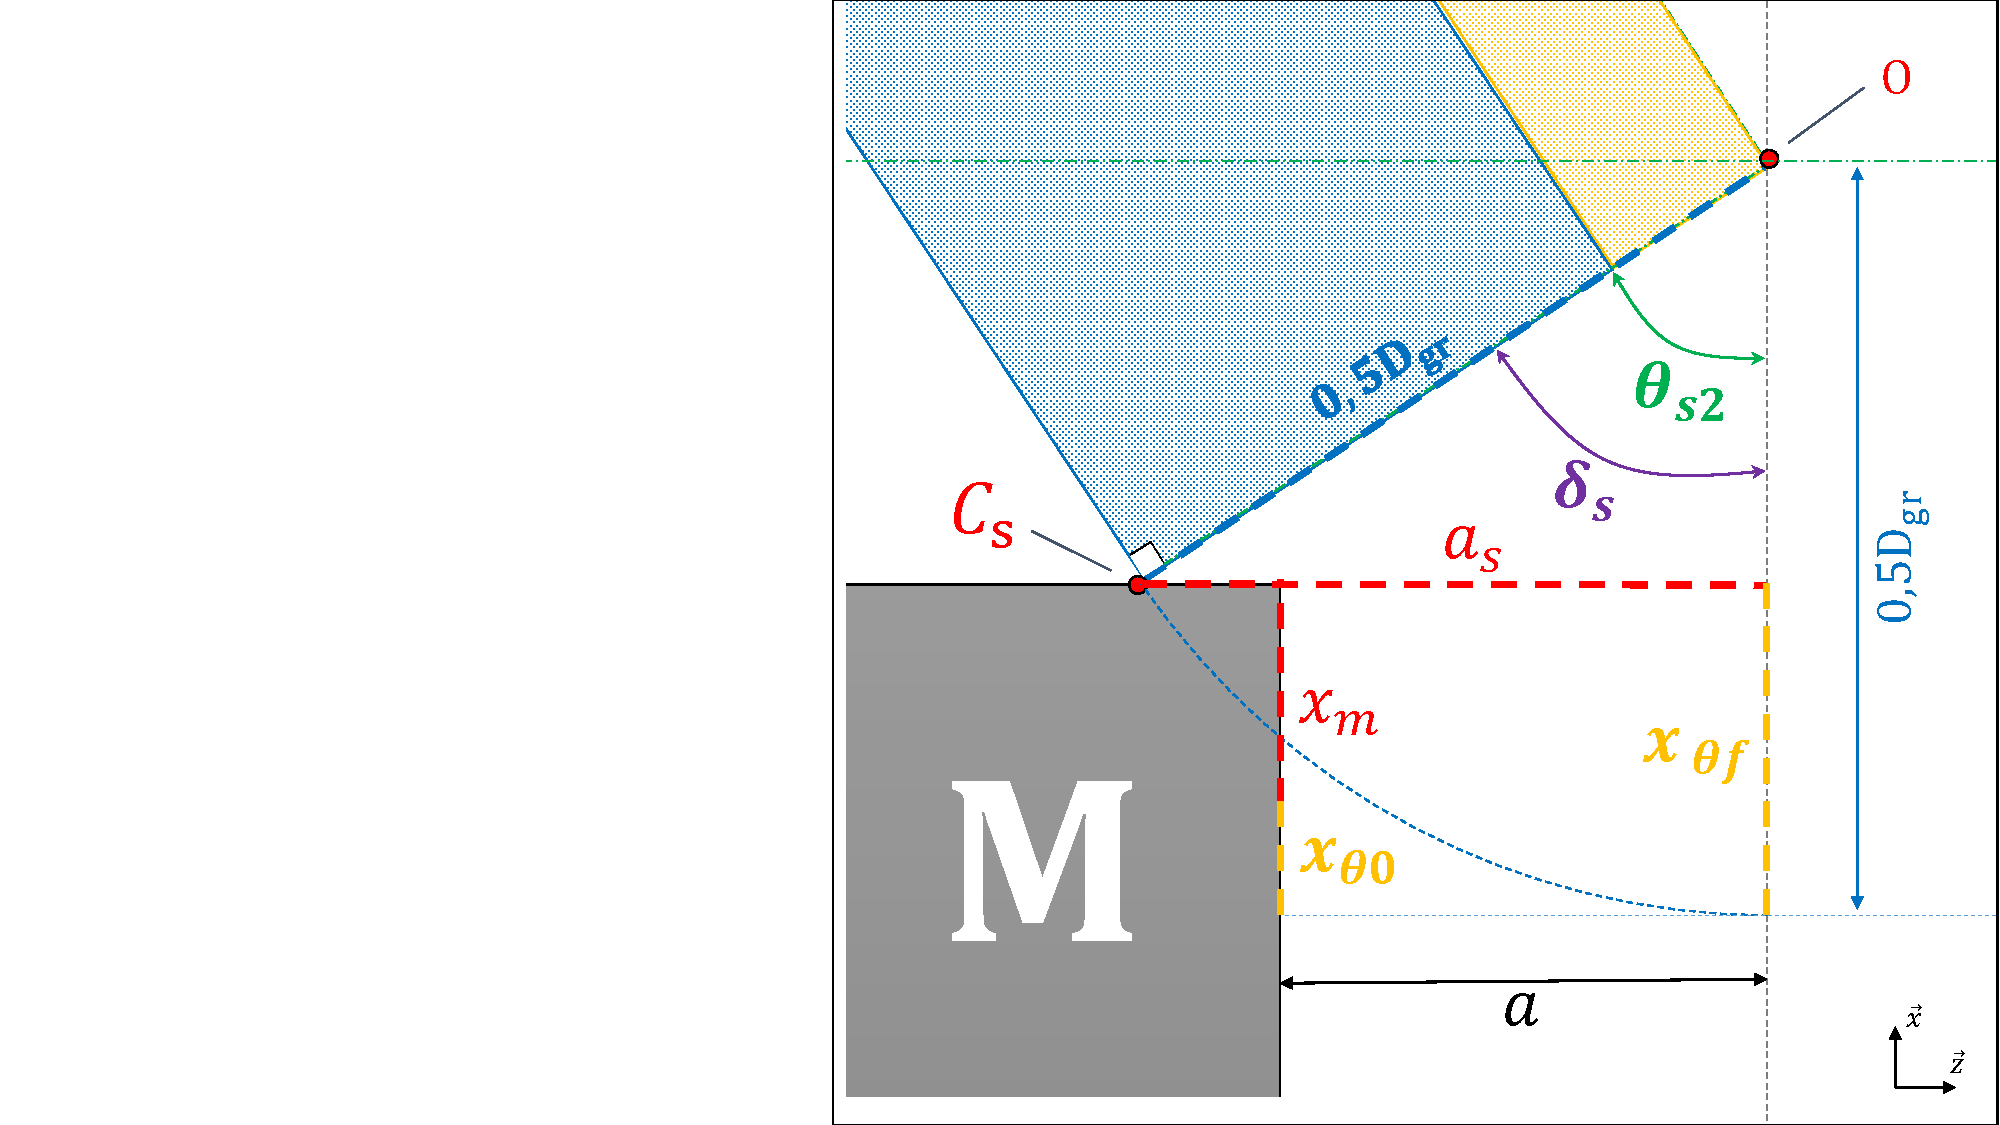
\includegraphics[trim={14cm 0cm 0cm 0cm},clip,width=.99\textwidth]{../Chap6/Figure/cinematique_pliage_VH_lacher_calculs_saut.pdf}
         \label{fig:cinematique_pliage_VH_lacher_calculs_saut_égal}}
   \end{minipage}\par\medskip
   \centering
   \subfloat[]{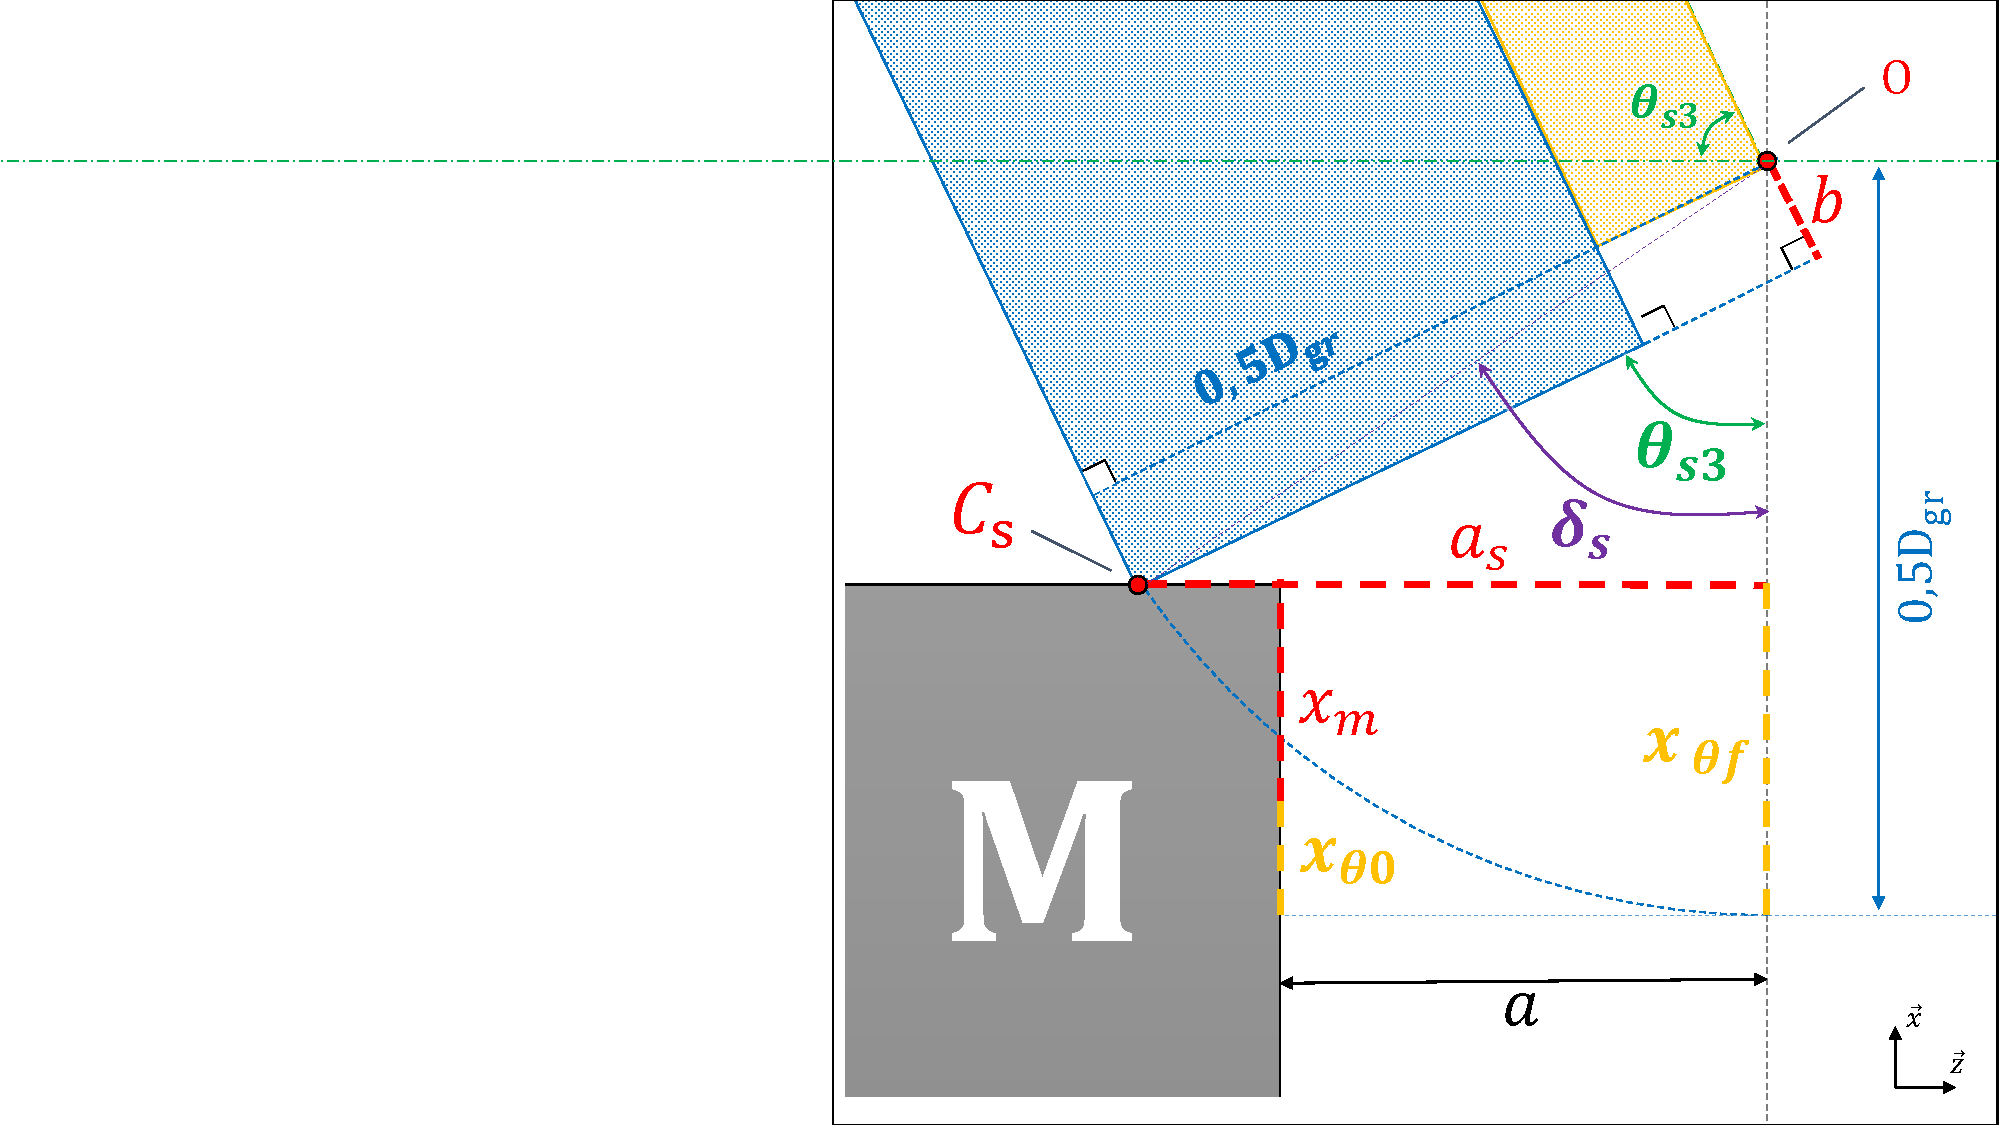
\includegraphics[trim={14cm 0cm 0cm 0cm},clip,width=.5\textwidth]{../Chap6/Figure/cinematique_pliage_VH_lacher_calculs_saut_grand.pdf}
      \label{fig:cinematique_pliage_VH_lacher_calculs_saut_grand}}
   \caption{Configuration du contact supérieur pour (a):$b=b_1$, (b):$b=0$ et (c):$b=b_3$}
   \label{fig:cinematique_pliage_VH_lacher_calculs_saut}
\end{figure}
%%%%%%%%%%%%%%%%


Le système d'équations  $S_{sup}$(\ref{eq:S_ap}) prédit alors le comportement de $\theta$ durant le contact supérieur, en fonction du déplacement $x_m$ de M, pour les trois cas de figures décrits précédemment. Il est expérimentalement difficile de se retrouver dans le cas de figure où $b=0$. Une faible variation de $b$ peut en effet engendrer une différence dans la cinématique de l'évolution de $\theta$ et donc une corrélation avec un modèle devient plus difficile. Il serait néanmoins possible de réduire l'incertitude sur $b$ en passant par des méthodes de fabrication avec des tolérances plus précises.

Le comportement statique n'est pas nécessaire pour extraire les paramètres de sortie du système d'équations $S_{sup}$. En effet, la condition statique imposant $x_{0,vh}$ intervient pour fixer le bras de levier initial $a$ en fonction $K_{VH}$ dans le respect de $\Delta\theta$ en contact latéral. Le tube T100p ayant été caractérisé précédemment en fonction de son angle de flexion, on peut en extraire sa raideur pour les deux valeurs d'angles aux bornes de l'intervalle $\Delta\theta$. Cela permet alors de déduire $x_{\theta 0}$ et $a$ à partir des systèmes d'équations \ref{eq:x_0f} - \ref{eq:equilibre_statique} et \ref{eq:f} - \ref{eq:xt}. Ces paramètres seront alors des données d'entrée dans le calcul des paramètres de sortie du système d'équation $S_{sup}$. On doit s'assurer par ailleurs de respecter la condition décrite dans l'inéquation \ref{eq:theta_max_av_saut} si on souhaite rester en contact latéral jusqu'à $x_m=x_{0,vh}$.

En résumé, les systèmes d'équations \{\ref{eq:x_0f} - \ref{eq:equilibre_statique}\},  \{\ref{eq:f} - \ref{eq:xt}\} et \ref{eq:S_ap} permettent de prédire le comportement statique et cinématique de l'{OBVH} durant les oscillations de M, en supposant que le contact M-VH soit permanent quel que soit $x_m$.\\
%%%%%%%%%%%%%%%%%%%%%%%%%%%%%%%%%%%%
\begin{subnumcases}{S_s~~}
   $$
   ~~~~~~~~~~~~~~~~~~~~ x_m = x_{\theta f} - x_{\theta 0}
   $$
   \label{eq:xm_saut}\\
   $$ b\ne0 \left\{
    \begin{array}{l}
   a_{s}\ = \frac{D_{gr}}{2}\sin(\theta_{s1}) + b\cos(\theta_{s1}) \\
   x_{\theta f} = \dfrac{D_{gr}}{2}\ \biggl(1-\cos(\theta_{s1})\biggr) + b\sin(\theta_{s1})\\
    \end{array}
   \right.$$
   \label{eq:saut_petit_et_grand}\\
   $$ b=0 \left\{
    \begin{array}{l}
   a_{s}\ = \frac{D_{gr}}{2}\sin(\theta_{s2}) \\
   x_{\theta f} = \dfrac{D_{gr}}{2}\ \biggl(1-\cos(\theta_{s2})\biggr) \\
    \end{array}
   \right.$$
   \label{eq:saut_egal}
   \end{subnumcases} 
   \label{eq:S_ap}